% Informal research notes for collaborators, 2026-11-18. Every number traces to a file in
% contrib/markerless_d9_d10/ of the cd-conjecture repository (README.md, REFEREE.md, certificate/, data/),
% named in a comment where it appears. Figures figU1-3.pdf are made by make_figs.py in this folder.
\documentclass[11pt]{article}
\usepackage[margin=1in]{geometry}
\usepackage{amsmath,amssymb}
\usepackage{graphicx}
\usepackage{booktabs}
\usepackage[font=small,labelfont=bf]{caption}
\usepackage[compact]{titlesec}
\usepackage[colorlinks=true,linkcolor=blue,citecolor=blue,urlcolor=blue]{hyperref}
\setlength{\textfloatsep}{14pt plus 2pt minus 4pt}

\newcommand{\ket}[1]{|#1\rangle}
\newcommand{\bra}[1]{\langle #1|}
\newcommand{\Kt}{\tilde K}
\newcommand{\Eu}{E_{\rm u}}
\newcommand{\hc}{\mathrm{h.c.}}

\begin{document}
\begin{center}
{\Large Unbounded central charge from ten states per site: notes}\\[6pt]
18 November 2026
\end{center}

% =============================================================================================
\section{The question}

The central charge $c$ of a critical chain counts its gapless degrees of freedom; it fixes the finite-size correction to the ground-state energy and the low-temperature specific heat~\cite{BloteCardyNightingale,Affleck86}. Latorre and Sierra conjectured~\cite{LatorreSierra} that a translation-invariant chain with nearest-neighbour interactions and $d$ states per site, whose low-energy theory is a unitary CFT, has
\begin{equation}
c\le d-1 .
\label{eq:cd}
\end{equation}
The $SU(d)$ permutation chains saturate it: they flow to $SU(d)_1$, with $c=d-1$~\cite{Sutherland,AffleckNPB}.

The intuition is a counting of states, but the counting does not force Eq.~\eqref{eq:cd}. A CFT with sectors of central charge $c_a$ and velocity $v_a$ has entropy density
\begin{equation}
s=\frac{\pi T}{3}\sum_a\frac{c_a}{v_a},
\label{eq:entropy}
\end{equation}
and on the lattice $s\le\ln d$. This constrains $c$ only if the conformal regime extends to temperatures of order the velocities, all of them of order the couplings. A mode that is slow on the lattice scale costs almost no entropy, and $c$ does not care how slow a mode is.

Free fermions that hop $b$ sites at a time,
\begin{equation}
H=-t\sum_x\big(c^\dagger_{x+b}c_x+\hc\big),
\label{eq:bhop}
\end{equation}
have the band $-2t\cos bk$ with $2b$ Fermi points: $b$ interpenetrating chains, and $c=b$ at $d=2$. Any shorter-range hopping of comparable strength removes the extra Fermi seas. So the question is whether nearest-neighbour interactions can generate hopping over $b$ sites with nothing shorter-ranged competing. For large $b$ one cannot tune all the shorter hoppings away; the lattice has to forbid them kinematically.

These notes describe a chain that does this with $d=10$. It orders into a soliton lattice whose period $b=n+1$ is set by a chemical potential for the solitons, and the $n$ other sites of a period hold hard-core bosons in $n$ exactly flat bands. Charge moves only when the solitons of neighbouring cells virtually excite each other, and then by exactly one period, which gives an $n$-band metal with $2n$ Fermi points. A dilute gas of holes lets the lattice float and adds one mode: $c=n+1$, worked out for $n=9,10,11,12,14,16,20$ ($c=10>9$ at $n=9$). The argument is perturbation theory, controlled for two cells, followed by weak-coupling bosonization, with several inputs assumed rather than derived. It is not a proof, and no central charge has been measured.

% =============================================================================================
\section{Ten states and the Hamiltonian}

A site is in one of ten states [Fig.~\ref{fig:scheme}(a)]: four matter states $L_a$, $R_a$, with an orientation $L$ or $R$ and the occupation $a\in\{0,1\}$ of a hard-core boson of charge one; a neutral kink $K$; kinks of charge $\pm\tfrac12$ in a bright ($K_\pm$) or a dark ($\Kt_\pm$) internal state; and a hole $\varnothing$. The orientations form domains. A kink is a site-centred wall with $L$ sites on its left and $R$ sites on its right, and it moves by trading places with a neighbour and flipping that neighbour's orientation,
\begin{equation}
\ket{L_a}\ket{\kappa}\;\longleftrightarrow\;\ket{\kappa}\ket{R_a},
\label{eq:move}
\end{equation}
for every kink state $\kappa$. The opposite walls, where an $R$ domain meets the next $L$ domain or kink, are bond-centred antikinks. A unit cell is the stretch between two antikinks. It reads $L_{a_0}\cdots L_{a_{j-1}}\,\kappa\,R_{a_j}\cdots R_{a_{n-1}}$, with $n$ matter sites and one kink at position $j\in\{0,\dots,n\}$, so $b=n+1$ sites. A kink at position $j$ sits just to the left of matter site $j$.

\begin{figure}[t]
\centering
\begin{minipage}[c]{0.46\textwidth}
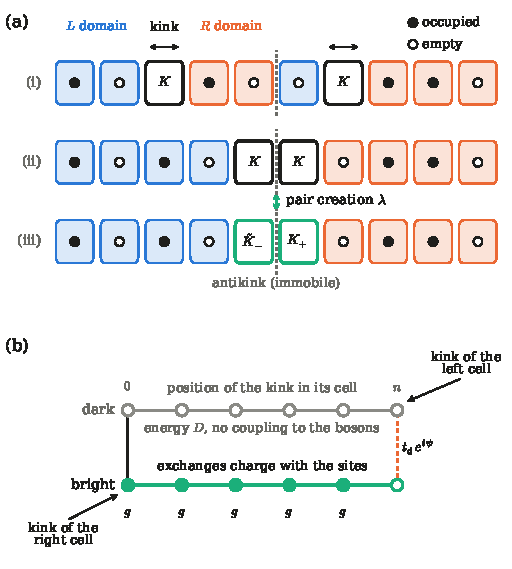
\includegraphics[width=\linewidth]{figU1.pdf}
\end{minipage}\hfill
\begin{minipage}[c]{0.51\textwidth}
\caption{\label{fig:scheme}(a) Two unit cells with $n=4$; filled and open circles are occupied and empty sites. (i) Each cell holds one kink, which moves by Eq.~\eqref{eq:move}; the antikink between the cells (dashed) does not move. (ii) Two kinks touch only when the left one is at the right edge of its cell and the right one at the left edge of its own. (iii) There they can turn into a pair of kinks of charge $\mp\tfrac12$. (b) The states of a charged kink in its cell, Eq.~\eqref{eq:Hs}. A bright kink exchanges charge with the site to its right (amplitude $g$); a dark kink, at extra energy $D$, does not. The kink of the left cell is created dark at the right edge and turns bright only at the left edge, where the kink of the right cell is created. The weak link $t_d$ closes the loop and threads a flux through it.}
\end{minipage}
\end{figure}

The Hamiltonian is $H=\sum_ih_{i,i+1}$, with
\begin{equation}
h=J\,\mathcal E(h_9)-t\sum_{x\ne\varnothing}\big(\ket{x\,\varnothing}\bra{\varnothing\,x}+\hc\big)-\frac{\mu_h}{2}\big(\bar P_\varnothing\otimes1+1\otimes\bar P_\varnothing\big),
\label{eq:h10}
\end{equation}
where $\bar P_\varnothing=1-P_\varnothing$ and $\mathcal E(h_9)$ acts as $h_9$ when neither site is a hole and vanishes otherwise. On the nine other states
\begin{equation}
h_9=w+\tfrac12\big(o\otimes1+1\otimes o\big)+U\,\Pi_{LR},
\label{eq:h9}
\end{equation}
\begin{align}
w={}&-\sum_a\Big[\ket{L_aK}\bra{KR_a}+\sum_{s=\pm}z_s(a)\Big(\ket{L_aK_s}\bra{K_sR_a}+e^{i\phi_s}\ket{L_a\Kt_s}\bra{\Kt_sR_a}\Big)\Big]\nonumber\\
&-\sum_s\sum_{y\ne L_0,L_1}\ket{y\,\Kt_s}\bra{y\,K_s}
-t_d\sum_se^{i\psi_s}\sum_{y\ne R_0,R_1}\ket{\Kt_s\,y}\bra{K_s\,y}\nonumber\\
&+g\,\ket{K_+R_0}\bra{K_-R_1}
+\lambda\Big(e^{-i\pi/4}\ket{\Kt_-K_+}+e^{i\pi/4}\ket{\Kt_+K_-}\Big)\bra{KK}+\hc,\label{eq:w}\\[2pt]
o={}&\nu\sum_\kappa P_\kappa+\Delta\sum_s\big(P_{K_s}+P_{\Kt_s}\big)+D\sum_sP_{\Kt_s}+f\sum_\ell q(\ell)\,P_\ell ,\label{eq:o}
\end{align}
with the Hermitian conjugate applied to all of $w$, $z_+(a)=1$, $z_-(a)=(-1)^a$, $\phi_+=0$, $y$ running over the non-hole states with the stated exclusions, $\kappa$ over the five kink states, $P_\ell$ the projector on state $\ell$ and $q(\ell)$ its charge [$q(L_a)=q(R_a)=a$, $q(K)=0$, $q(K_\pm)=q(\Kt_\pm)=\pm\tfrac12$], and $\Pi_{LR}$ the projector on the pairs $(L_a,R_{a'})$.

The first line of $w$ is the kink motion~\eqref{eq:move}, with a sign $(-1)^a$ for charge $-\tfrac12$ and a phase $e^{i\phi_s}$ for a dark kink. The second turns a bright kink dark and back, with amplitude one at the left edge of its cell and the small amplitude $t_d$ at the right edge. The third is the charge exchange, a bright kink absorbing or emitting the boson on the site to its right, and the pair creation of a dark and a bright kink of opposite charges from two touching neutral kinks. $\nu$ is a chemical potential for kinks, $\Delta$ and $D$ the extra costs of a charged and of a dark kink, $f$ a chemical potential for the charge, and $U\ge0$ the cost of an $L\to R$ wall without a kink. Through $\mathcal E$, every term of $h_9$, the on-site energies included, acts only between sites in contact.

Three properties hold exactly, for all couplings.
\emph{(i)} Let $F$ count the $L\to R$ walls without a kink, the adjacent pairs $(L,R)$ once the holes are deleted. The kink motion maps $x\,L_a\kappa\,y$ to $x\,\kappa R_a\,y$; it destroys the pairs $(x,L_a)$, $(L_a,\kappa)$, $(\kappa,y)$ and creates $(x,\kappa)$, $(\kappa,R_a)$, $(R_a,y)$, none of the form $(L,R)$ whatever $x$ and $y$ are. No other term changes an orientation, and a hole hop does not change the configuration with holes deleted. So $[H,F]=0$, and the sector $F=0$, with one kink on every $L\to R$ wall, is invariant; it is not imposed by an energy penalty.
\emph{(ii)} Let $B_i=1$ if site $i$ is not an $L$ and site $i+1$ is not an $R$, which is the case exactly at an antikink. The kink motion on sites $(i,i+1)$ keeps $B_i=0$ and does not change $B_{i\pm1}$, so the antikinks do not move and the cells are rigid. For $F=0$ each cell holds exactly one kink, unless there are none.
\emph{(iii)} A neutral kink moves the same way whatever the occupations of the sites it passes; charged kinks feel them only through the signs $z_-(a)$.
The charge and the number of holes are conserved too. An exhaustive check of all transitions on rings (nine states up to length 7, ten up to 6, and ten up to 5 for the rigidity of the cells) finds no violation of (i), (ii) or these conservation laws. % data/ring_checks_bond9_L7.json, data/ring_checks.json, ring_checks_contact.log (F only); referee/ring_invariants_L7_L6.log (F,Q,heads,occ; B_i to L=7 at d=9, squeezed pattern to L=5 at d=10); referee/addendum_checks.log

% =============================================================================================
\section{The soliton lattice and flat bands}\label{sec:lattice}

Without holes $H=J\sum_ih_9$, and we set $J=1$. At $\lambda=0$ no charged kinks are created, and for $\Delta>0$ they cost energy. In the sector $F=0$ with neutral kinks, $H$ is then a sum over cells, and in each cell the kink is a particle in a box of $b$ positions,
\begin{equation}
\chi_j=\sqrt{\tfrac{2}{b+1}}\,\sin\tfrac{\pi(j+1)}{b+1},\qquad E_{\rm cell}=\nu-2\cos\tfrac{\pi}{b+1},
\label{eq:box}
\end{equation}
with amplitude $\alpha\equiv\chi_0=\chi_n$ at either edge. Cells of lengths $b_c$ have total energy $\sum_cb_c\,e_{b_c}$, with the energy per site
\begin{equation}
e_b=\frac1b\Big[\nu-2\cos\frac{\pi}{b+1}\Big],
\label{eq:eb}
\end{equation}
while stretches without a kink cost $0$ or $U$. So if a period $b$ minimizes $e_b$ and $e_b<0$, the uniform lattice of period $b$ is the ground state. The zero-point energy $\zeta_b=2[1-\cos(\pi/(b+1))]$ is convex in $b$, and period $b$ wins on the window
\begin{equation}
2-\delta_{b-1}<\nu<2-\delta_b,\qquad \delta_b=(b+1)\,\zeta_b-b\,\zeta_{b+1},
\label{eq:window}
\end{equation}
with $b\simeq\pi[3/(2-\nu)]^{1/2}$ at large $b$: the chemical potential sets the spacing. For $b=10$ ($n=9$) the window is $1.7503<\nu<1.7903$, that is $\pm0.020$ around $\nu=1.7703$, where the period $b=11$ is higher by $1.8\times10^{-4}$ per site and the first excitation of a kink in its cell costs $0.236$. % data/selector.json; window from Eq. (window)

By property (iii), all $2^n$ occupation patterns of a cell are exactly degenerate at fixed charge. Each cell carries $n$ fermion orbitals with no dispersion and no interaction: $n$ flat bands.

% =============================================================================================
\section{How charge moves}\label{sec:charge}

Pair creation acts only where two neutral kinks touch [Fig.~\ref{fig:scheme}(a)(ii)], with amplitude $\alpha^2$ in the ground state of the two cells, and it lifts both kinks into charged states. Nothing happens at first order. At order $\lambda^2$ a pair is created and annihilated without touching the bosons, which only shifts the energy. Odd orders in $g$ change the charge of the matter and vanish within the flat bands. At order $\lambda^2g^2$ a pair is created, each kink exchanges one unit of charge with a site of its own cell, and the pair annihilates: a boson has moved to the next cell. This is a fourth-order superexchange in which the virtual particles are fractionally charged solitons.

After a gauge transformation that absorbs the signs $z_-(a)$ into the parity of the occupations passed, a kink of charge $s/2$ is a particle on the graph of Fig.~\ref{fig:scheme}(b), with bright states $\ket j$ and dark states $\ket{\tilde\jmath}$, $j=0,\dots,n$:
\begin{align}
H_s={}&\sum_{j=0}^n\Big(m\ket j\bra j+(m+D)\ket{\tilde\jmath}\bra{\tilde\jmath}\Big)
-\sum_{j=0}^{n-1}\Big(\ket{j+1}\bra j+e^{i\phi_s}\ket{\widetilde{j+1}}\bra{\tilde\jmath}+\hc\Big)\nonumber\\
&-\Big(\ket{\tilde0}\bra0+t_de^{i\psi_s}\ket{\tilde n}\bra n+\hc\Big),
\label{eq:Hs}
\end{align}
where $m=\Delta+2\cos[\pi/(b+1)]$ is the energy of a bright kink above the vacuum of its cell. The left kink of a pair is created in $\ket{\tilde n}$ and the right one in $\ket0$; a bright kink at $j\le n-1$ exchanges charge with site $j$. The graph is a ring threaded by the flux $\psi_s-n\phi_s$. We take $\phi_-=\pi/(2n)$, $\psi_-=\pi$ and $\psi_+=\pi/2$, so that both charges see flux $\pi/2$.

The propagator at zero energy of a pair with charge $s/2$ in the left cell and $s'/2$ in the right cell is
\begin{equation}
R_{ss'}=\big(H_s\otimes1+1\otimes H_{s'}\big)^{-1}.
\label{eq:R}
\end{equation}
With $\Pi^L_j=\ket j\bra j\otimes1$, $\Pi^R_j=1\otimes\ket j\bra j$ and $\ket\Omega=\ket{\tilde n}\otimes\ket0$, define the $n\times n$ matrices
\begin{align}
T_{jj'}&=\frac{i}{\beta^2}\,\bra\Omega R_{-+}\Pi^L_jR_{++}\Pi^R_{j'}R_{+-}+R_{-+}\Pi^R_{j'}R_{--}\Pi^L_jR_{+-}\ket\Omega,\label{eq:T}\\
\mu^L_{jj'}&=-\frac{1}{\beta^2}\,\bra\Omega R_{-+}\Pi^L_jR_{++}\Pi^L_{j'}R_{-+}-R_{+-}\Pi^L_{j'}R_{--}\Pi^L_jR_{+-}\ket\Omega,\label{eq:muL}\\
\mu^R_{jj'}&=-\frac{1}{\beta^2}\,\bra\Omega R_{+-}\Pi^R_jR_{++}\Pi^R_{j'}R_{+-}-R_{-+}\Pi^R_{j'}R_{--}\Pi^R_jR_{-+}\ket\Omega,\label{eq:muR}
\end{align}
and $\mu=\mu^L+\mu^R$. Here $\beta$ is the amplitude for a dark kink to cross its cell,
\begin{equation}
\beta=\frac{1}{u_{n+1}},\qquad u_0=1,\quad u_1=m+D,\quad u_{k+1}=(m+D)\,u_k-u_{k-1},
\label{eq:beta}
\end{equation}
which falls roughly like $(m+D)^{-(n+1)}$. The two terms of $T$ are the two orders in which the kinks exchange charge. The two terms of $\mu^{L}$ (or $\mu^R$) are the left (right) kink absorbing first, as charge $-\tfrac12$, or emitting first, as charge $+\tfrac12$; they have opposite signs because the bosons have become fermions. The factor $i$ comes from the phases of the pair creation, and the overall signs were fixed by comparison with the microscopic Hamiltonian. With fermions $c_{I,j}$ ($I$ the cell, $j$ the site in it), the Hamiltonian at order $\lambda^2g^2$ is, up to a constant,
\begin{equation}
H_{\rm eff}=\sum_I\Big[c_I^\dagger\big(\Eu\,\mu+f\big)c_I+\Eu\big(c_I^\dagger\,T\,c_{I+1}+\hc\big)\Big],\qquad \Eu=\lambda^2\alpha^4\beta^2g^2 ,
\label{eq:Heff}
\end{equation}
with $\alpha^4$ the probability that two neutral kinks touch.

$H_{\rm eff}$ is exactly quadratic. Each process moves one boson, or moves it and puts it back, and by property (iii) its amplitude depends on the other occupations only through the signs $(-1)^a$ picked up by the kinks of charge $-\tfrac12$. Their product is, up to a sign that does not depend on the occupations, the parity of the bosons strictly between the site the boson leaves and the site it reaches, which is the Jordan--Wigner string, and hard-core bosons that hop with their string attached are free fermions. Exact perturbation theory in the microscopic Hamiltonian, on two cells ($n\le4$) and on a ring of three cells ($n\le2$), confirms this: the order-$\lambda^2g^2$ term is a constant plus a fermion bilinear, and its blocks agree with Eqs.~\eqref{eq:T}--\eqref{eq:muR}, both to $4\times10^{-11}$ of the hopping or better at well-conditioned couplings. % data/two_cell_checks.json (max 3.7e-11 Gaussian, 3.1e-11 blocks; n=3,D=8,td=0 point is 1.5e-8, ill-conditioned), data/ring_three_cells.json; referee item3_n4.json, item3_rings.json (2.4e-11); REFEREE.md item 3

Why is the dark state needed? For $t_d=0$ and $D\to\infty$ the left kink crosses its cell instantly and turns bright at the left edge, where the right kink is created, so both kinks explore their cells from the left edge. Writing each propagator as $\int_0^\infty d\tau\,e^{-\tau E}$, the two terms of $T$ combine into
\begin{equation}
T_{jj'}\propto\int_0^\infty d\tau\,G_j(\tau)\,G_{j'}(\tau),\qquad
G_j(\tau)=\int_0^\tau d\tau'\,\bra0e^{-(\tau-\tau')H_{\rm br}}\ket j\bra j e^{-\tau'H_{\rm br}}\ket0,
\label{eq:gram}
\end{equation}
with $H_{\rm br}$ the bright part of Eq.~\eqref{eq:Hs}; $G_j(\tau)$ is the amplitude for a bright kink that starts at the left edge to exchange charge with site $j$ and be back there after imaginary time $\tau$. So $T$ is a matrix of overlaps, positive up to a phase, and at large but finite $D$ (still $t_d=0$), $T=e^{i\theta}(S+iA)$ with $S$ positive and $A$ Hermitian; at small $D$ the positivity of $S$ can fail. Charge hops by exactly one period with a positive $n\times n$ matrix of amplitudes: the long-range hopping of Eq.~\eqref{eq:bhop}. Without the dark state the kinks, created where their cells meet, would explore them in mirror-image order, $T=\mathcal JS$ with $\mathcal J$ the reflection $j\to n-1-j$, and orbital $j$ of one cell would pair with orbital $n-1-j$ of the next in a dimerized chain of Su--Schrieffer--Heeger type~\cite{SSH}, gapped unless $j$ is central. A seven-state chain without dark states indeed has no Fermi points out of four at $n=2$ and two out of six at $n=3$ (zero field, one set of couplings: an explanation, not a no-go theorem). We expect dark states to be needed for both charges: otherwise $\mu$ would not cancel at $t_d=0$ and would exceed the hopping by $\beta^{-2}$ (an estimate, not computed). % data/seven_check.json; seven_letter_negative/

% =============================================================================================
\section{An \texorpdfstring{$n$}{n}-band metal}\label{sec:metal}

The Bloch Hamiltonian, with $k$ conjugate to the cell index, is
\begin{equation}
h(k)=\mu+f/\Eu+T\,e^{ik}+T^\dagger e^{-ik},
\label{eq:bloch}
\end{equation}
and the Fermi momenta are the zeros of $\det h(k)$. At $t_d=0$ the graph has no loop, $\mu$ vanishes (the two charges see the same graph and contribute with opposite fermionic signs), and $T=e^{i\theta}(S+iA)$. Then, at $f=0$, every band crosses zero energy. With $z=e^{ik}$, $z^n\det h(k)=\det(Tz^2+T^\dagger)$ is a polynomial of degree $2n$, and if $(Tz^2+T^\dagger)v=0$ then
\begin{equation}
z^2=-\frac{v^\dagger T^\dagger v}{v^\dagger Tv}=-e^{-2i\theta}\,\frac{\sigma-i\eta}{\sigma+i\eta},\qquad \sigma=v^\dagger Sv>0,\quad \eta=v^\dagger Av\in\mathbb R,
\label{eq:unitcircle}
\end{equation}
so $|z|=1$. All $2n$ zeros lie on the unit circle, for any positive $S$, however unequal its eigenvalues.

They are very unequal. A boson deep inside a cell is reached only by a kink that has tunnelled far from the edge at a cost $m$, so the eigenvalues of $S$, which set the band widths and Fermi velocities, form a geometric ladder,
\begin{equation}
v_a\simeq v_1\,r^{\,a-1},\qquad r\approx10^{-2.74}\approx1/550,
\label{eq:ladder}
\end{equation}
for $m=4$ and each $n$ of Table~\ref{tab:cases} [Fig.~\ref{fig:cd}(b)]. % data/velocity_ladders.json (fit slopes -2.735 to -2.736)

At $t_d=0$ the Fermi points come in pairs $k+\theta\leftrightarrow-(k+\theta)$, and two fermions at opposite points of one band can scatter into opposite points of another, which gaps weakly coupled chains~\cite{BalentsFisher,LinBalentsFisher}. The link $t_d$ closes the path of a charged kink into a loop with flux $\pi/2$, breaking time reversal and making the Fermi momenta generic ($T$ becomes real up to a phase, $\mu$ imaginary and, to leading order, proportional to $t_d$). It also lets a kink into its cell from the wrong edge, a mirror-image contribution, so it must stay below the narrowest band. The low-energy theory needs $2n$ distinct Fermi momenta $k_i$ with
\begin{equation}
k_i+k_j\ne k_l+k_{l'}\pmod{2\pi}\qquad\text{for }\{i,j\}\ne\{l,l'\},
\label{eq:nonres}
\end{equation}
$i=j$ allowed. Table~\ref{tab:cases} lists couplings for which this holds, for $n$ from 9 to 20. The Fermi momenta were bracketed with rigorous error bounds and cross-checked at $n=9$ and 10 by an independent evaluation of Eqs.~\eqref{eq:T}--\eqref{eq:muR} at 230 and 260 significant digits. At $n=9$ the eighteen Fermi momenta are separated by more than $0.0168$ and the pair momenta by more than $8.8\times10^{-5}$ (Fig.~\ref{fig:bands}). The couplings $g$ and $\lambda$ are small enough that two-cell estimates of the higher orders cannot move any Fermi momentum out of its bracket; they are sufficient for this, not optimized. % certificate/root_certificate_n*.json, finite_budget_n*.json; data/crosscheck_certificate_n9.json, _n10.json

\begin{table}[t]
\centering
\caption{\label{tab:cases}Couplings with $2n$ Fermi points obeying Eq.~\eqref{eq:nonres}: $m=4$, $D=1000$, fluxes as in Sec.~\ref{sec:charge}, $\nu$ at the middle of the window~\eqref{eq:window}, and the values listed. $\delta k$, $\delta K$: lower bounds on the smallest separation of the Fermi momenta and of the pair momenta. Last columns: slowest over fastest velocity, and the scale of Eq.~\eqref{eq:Heff} in units of the kink hopping.}
\smallskip
\small
\begin{tabular}{rcccccccc}
\toprule
$n$ & $t_d/\beta$ & $f/\Eu$ & $g$ & $\lambda$ & $\delta k$ & $\delta K$ & $\log_{10}(v_n/v_1)$ & $\log_{10}\Eu$\\
\midrule
9 & $2^{-35}$ & $2^{-83}$ & $2^{-163}$ & $2^{-359}$ & 0.01680 & $8.83\times10^{-5}$ & $-21.9$ & $-378$\\
10 & $2^{-42}$ & $2^{-92}$ & $2^{-177}$ & $2^{-388}$ & 0.01541 & $8.79\times10^{-5}$ & $-24.7$ & $-410$\\
11 & $2^{-48}$ & $2^{-101}$ & $2^{-192}$ & $2^{-419}$ & 0.01516 & $4.87\times10^{-5}$ & $-27.4$ & $-444$\\
12 & $2^{-56}$ & $2^{-111}$ & $2^{-207}$ & $2^{-448}$ & 0.01479 & $3.09\times10^{-6}$ & $-30.2$ & $-477$\\
14 & $2^{-68}$ & $2^{-129}$ & $2^{-235}$ & $2^{-506}$ & 0.01472 & $6.49\times10^{-7}$ & $-35.7$ & $-541$\\
16 & $2^{-84}$ & $2^{-147}$ & $2^{-265}$ & $2^{-566}$ & 0.01442 & $3.43\times10^{-6}$ & $-41.2$ & $-607$\\
20 & $2^{-112}$ & $2^{-184}$ & $2^{-323}$ & $2^{-683}$ & 0.01405 & $1.60\times10^{-6}$ & $-52.2$ & $-737$\\
\bottomrule
\end{tabular}
% t_d/beta = 2^-e, f/E_u = 2^-F: supplement Table S2 / README; g, lambda: certificate/finite_budget_n*.json;
% delta k, delta K: root_certificate_n*.json (delta2_lower, delta4_lower), truncated; velocities: data/velocity_ladders.json;
% log10 E_u = log10(lambda^2 alpha^4 beta^2 g^2), with log10_beta from certificate_n*.json (-30.02 at n=9): -377.99, -410.11, -444.01, -476.70, -540.82, -607.32, -737.21.
\end{table}

\begin{figure}[t]
\centering
\begin{minipage}[t]{0.49\textwidth}
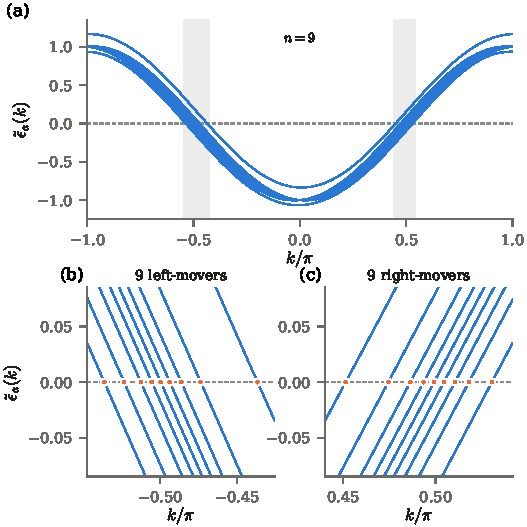
\includegraphics[width=\linewidth]{figU2.pdf}
\caption{\label{fig:bands}Bands for $n=9$ (couplings of Table~\ref{tab:cases}). (a) Eigenvalues of $\tfrac12S^{-1/2}h(k)S^{-1/2}$, which vanish where the bands do but are all of order one. (b), (c) The shaded windows: eighteen distinct Fermi points.}
\end{minipage}\hfill
\begin{minipage}[t]{0.49\textwidth}
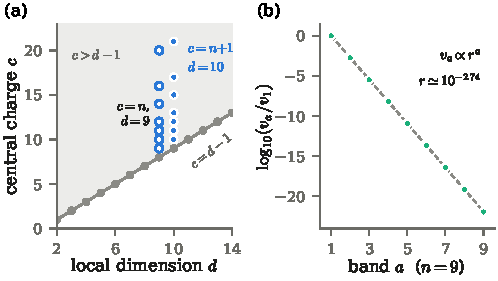
\includegraphics[width=\linewidth]{figU3.pdf}
\caption{\label{fig:cd}(a) Predicted $c$ against states per site: $c=n+1$ with ten states (filled), $c=n$ with nine and a pinned lattice (open); gray, $c=d-1$ ($SU(d)_1$ chains). (b) Band velocities at $n=9$, Eq.~\eqref{eq:ladder}.}
\end{minipage}
\end{figure}

% =============================================================================================
\section{Low-energy theory}

\subsection{An \texorpdfstring{$n$}{n}-component Luttinger liquid}\label{sec:LL}

Linearizing at the $2n$ Fermi points gives $n$ right- and $n$ left-moving fermions $\Psi_i$, a free theory with $c=n$. The microscopic chain adds interactions at orders $\lambda^2g^4$ and $\lambda^4$; for two cells, the estimates of Sec.~\ref{sec:metal} bound them far below every band width. The $U(1)$ forbids pairing terms. Translation by one cell conserves momentum modulo $2\pi$, and by Eq.~\eqref{eq:nonres} a quartic term $\Psi_i^\dagger\Psi_j^\dagger\Psi_{l'}\Psi_l$ with $k_i+k_j=k_l+k_{l'}$ has $\{i,j\}=\{l,l'\}$: only density--density terms $\rho_i\rho_j$ survive, and umklapp and interband pair tunnelling are excluded. Density--density terms are exactly marginal. They give an $n$-component Luttinger liquid with renormalized velocities and exponents~\cite{Haldane,Giamarchi} and
\begin{equation}
c=n .
\label{eq:cn}
\end{equation}

\subsection{Holes, and a floating lattice}

Without holes the soliton lattice is pinned: translation by one site is broken and the spectrum is $b$ identical copies, each with Eq.~\eqref{eq:cn}. Nine states thus already give $c=n>8$ for each $n$ of Table~\ref{tab:cases}, with translations broken. Holes restore them. A hole hop does not change the configuration with holes deleted, so the constraint stays invariant. For $J\ll t$ the holes form a fast free Fermi gas that sees the rest as a featureless background, as in the $J\to0$ limit of the $t$--$J$ chain~\cite{OgataShiba}: the eigenstates factorize into a wavefunction of the holes and one of the nine-state chain with the holes squeezed out, and to first order in $J$ each bond term of $h_9$ is multiplied by the probability $p$ that its two sites are in contact.

This is why the on-site energies must act only between sites in contact. The selection of the period, the flat bands and $H_{\rm eff}$ depend on ratios of the couplings in $h_9$, which survive only if every term is multiplied by the same $p$. An on-site energy acting regardless of the neighbours would keep its full value while the hopping is reduced; the cell energy would become $J[\nu-2p\cos(\pi/(b+1))]$, and at $n=9$ kinks would cost energy once $p<\nu/[2\cos(\pi/11)]=0.92$. With contact on-site energies the nine-state Hamiltonian becomes $pJh_9$, and Secs.~\ref{sec:lattice}--\ref{sec:LL} carry over with $J\to pJ$.

\begin{table}[t]
\centering
\caption{\label{tab:holes}Energy of one $n=9$ cell with $N_h$ holes on a ring, relative to the ring with no kink and divided by its value without holes ($-0.1487$), against the contact probability $p$ of the hole gas on the same ring.}
\smallskip
\begin{tabular}{lcccc}
\toprule
$N_h$ & 1 & 2 & 3 & 4\\
\midrule
$p$ & 0.900 & 0.802 & 0.710 & 0.626\\
ratio, $t/J=25$ & 0.902 & 0.805 & 0.714 & 0.630\\
ratio, $t/J=1$ & 0.940 & 0.865 & 0.786 & 0.708\\
\bottomrule
\end{tabular}
% data/mobile_selector_n9.json (contact); p from referee/addendum_checks.json part C
\end{table}

We checked this on one cell (Table~\ref{tab:holes}): its energy stays negative and at $t/J=25$ equals $p$ times its hole-free value to $0.7\%$, with a deviation that grows with $J/t$. This tests the sign and the uniformity of the rescaling for one cell without charged kinks, not competing periods at finite hole density, several cells, or pair creation with holes. The soliton lattice then floats on the hole gas, translation symmetry is restored, and the density mode of the holes adds one gapless boson:
\begin{equation}
c=n+1,
\label{eq:cn1}
\end{equation}
which exceeds $d-1=9$ for each $n$ of Table~\ref{tab:cases} [Fig.~\ref{fig:cd}(a)].

% =============================================================================================
\section{Counting of states, and the cost}

There is no conflict with the counting of states: the $n$ modes of a cell share the entropy $n\ln2$ of its flat bands, less than $\ln2$ per site, and Eq.~\eqref{eq:entropy} holds only below the smallest velocity. The cost is in the scales (Table~\ref{tab:cases}). At $n=9$ the gapless sector lies at $\Eu\approx10^{-378}$ of the microscopic couplings (times $p$ with holes) and the velocities span a further 22 orders of magnitude, with couplings sufficient for our estimates, not optimized. The steepness of the ladder is set by the kink gap $m$. This is an existence argument, far beyond numerical simulation.

The central charge is blind to velocities; the Casimir energy and the specific heat are not,
\begin{equation}
E_0(L)=e_0L-\frac{\pi}{6L}\sum_ac_av_a,\qquad \frac{C}{L}=\frac{\pi T}{3}\sum_a\frac{c_a}{v_a}.
\label{eq:casimir}
\end{equation}
The Casimir coefficient is dominated by the fastest band and stays of order $v_1$ as $n$ grows. The specific heat is dominated by the slowest band and grows like $1/v_n$, which is the statement that the conformal regime starts only below $T\sim v_n$. Whatever the lattice bounds has to involve the velocities, and the velocity-weighted sum $\sum_ac_av_a$ is the natural candidate.

% =============================================================================================
\section{What is assumed and what is open}

The prediction $c=n+1$ ($c=n$ without holes) rests on the following inputs, none established here.
\begin{enumerate}\setlength\itemsep{1pt}
\item The elimination of the massive sector (charged kinks, excitations of the neutral kink) is uniform in the length of the chain. It is controlled for two cells only; three-cell processes at order $\lambda^4$ are not computed, and the two-cell bound on higher orders in $\lambda$ rests on a contour estimate whose conditions we checked but whose constant we did not rederive.
\item The weakly interacting liquid is stable, including the non-quadratic terms of orders $\lambda^2g^4$ and $\lambda^4$.
\item At small $\lambda$ the uniform lattice of the selected period remains the ground state, against lattices with defects. At $\lambda=0$ this is exact.
\item The hole gas and the nine-state chain decouple at small but finite $J/t$, and how small is not quantified. The window in $\nu$ is $\pm0.020$ at $n=9$, about $13\%$ of the cell energy; the one-cell rescaling is uniform to $0.7\%$ at $t/J=25$ but off by 4 to $13\%$ at $t/J=1$, and a one-cell test cannot see the $1.8\times10^{-4}$ per site that separates neighbouring periods. Corrections of relative order $J/t$ to $T$ and $\mu$ must also fit within the tolerance of the Fermi-point analysis. One is already visible: $f$ acts only between sites in contact, so the hole gas gives a boson an energy that varies from site to site, by about $0.03\,(J/t)\,Jf$ in a cell with $n=3$. (The charge is conserved, so a field applied to every site regardless of contact would be a pure chemical potential and would not do this.) % REFEREE.md addendum item 4; referee/addendum_checks.json part D
\item There is no statement for all $n$: the couplings are worked out at $n=9,10,11,12,14,16,20$, with no obstruction seen to larger $n$.
\item No central charge has been measured.
\end{enumerate}

We do not know the smallest $d$ at which $c$ is unbounded. Nine states give $c=n$ with a pinned lattice. Each of the nine has a role in this mechanism, and without dark states the bands dimerize at the couplings we tried, but that is not a lower bound on $d$.

\medskip
\noindent\emph{Dictionary for the code:} $W=K$, $A=K_-$, $B=K_+$, $X_A=\Kt_-$, $X_B=\Kt_+$, $V=\varnothing$, the penalty $U$ is called $K$, and all charges are doubled.

% =============================================================================================
\begin{thebibliography}{99}\small\setlength\itemsep{0pt}
\bibitem{BloteCardyNightingale} H. W. J. Bl\"ote, J. L. Cardy, and M. P. Nightingale, Phys.\ Rev.\ Lett.\ \textbf{56}, 742 (1986).
\bibitem{Affleck86} I. Affleck, Phys.\ Rev.\ Lett.\ \textbf{56}, 746 (1986).
\bibitem{LatorreSierra} J. I. Latorre and G. Sierra, The $c$--$d$ conjecture, arXiv:2403.17242.
\bibitem{Sutherland} B. Sutherland, Phys.\ Rev.\ B \textbf{12}, 3795 (1975).
\bibitem{AffleckNPB} I. Affleck, Nucl.\ Phys.\ B \textbf{265}, 409 (1986).
\bibitem{SSH} W. P. Su, J. R. Schrieffer, and A. J. Heeger, Phys.\ Rev.\ Lett.\ \textbf{42}, 1698 (1979).
\bibitem{BalentsFisher} L. Balents and M. P. A. Fisher, Phys.\ Rev.\ B \textbf{53}, 12133 (1996).
\bibitem{LinBalentsFisher} H.-H. Lin, L. Balents, and M. P. A. Fisher, Phys.\ Rev.\ B \textbf{56}, 6569 (1997).
\bibitem{Haldane} F. D. M. Haldane, J. Phys.\ C \textbf{14}, 2585 (1981).
\bibitem{Giamarchi} T. Giamarchi, \emph{Quantum Physics in One Dimension} (Oxford University Press, 2004).
\bibitem{OgataShiba} M. Ogata and H. Shiba, Phys.\ Rev.\ B \textbf{41}, 2326 (1990).
\end{thebibliography}

\end{document}
